\documentclass[a4paper,12pt]{article}

\usepackage{graphicx}
\usepackage{geometry} % Modificar márgenes
\geometry{ % Especificación modificación márgenes
    a4paper,
    left=2cm,
    right=2cm,
    top=2cm,
    bottom=2cm
}
\usepackage[utf8]{inputenc}
\usepackage[spanish]{babel} % Paquete para escritura en español
\usepackage{float} % Etiqueta 'H' (mayus) en figuras (imágenes)
\usepackage{array} % Padding en tablas
\usepackage{url} % Etiqueta url en .bib
\usepackage{booktabs} % Manejo de caudros (tablas)
\usepackage[T1]{fontenc}    % Codificación de fuentes
\usepackage{csquotes}       % Paquete para comillas tipográficas

\begin{document}

\section{Material de apoyo}

Para la investigación sobre \textit{Colecciones en Java} (trabajo escrito) consultó los siguientes sitios en internet en su búsqueda confiable de información. La consulta a la API de Java fue recurrente para tener información fidedigna de cada interfaz y clase explorada, los demás sitios contienen información complementaria. Del mismo modo se muestran las clases consultadas en la realización del código fuente del programa de inscripción.

\subsection{API de Java}

\begin{itemize}
    \item Oracle. (2014). \textit{Interface Set$<$E$>$}. Java Platform Standard Edition 8 Documentation. Recuperado 14 de marzo de 2024, de\\https://docs.oracle.com/javase/8/docs/api/java/util/Set.html
    \item Oracle. (2014). \textit{Interface Map$<$K,V$>$}. Java Platform Standard Edition 8 Documentation. Recuperado 14 de marzo de 2024, de\\https://docs.oracle.com/javase/8/docs/api/java/lang/Map.html
    \item Oracle. (2014). \textit{Interface List$<$E$>$}. Java Platform Standard Edition 8 Documentation. Recuperado 14 de marzo de 2024, de\\https://docs.oracle.com/javase/8/docs/api/java/lang/List.html
    \item Oracle. (2014). \textit{Interface Collection$<$E$>$}. Java Platform Standard Edition 8 Documentation. Recuperado 14 de marzo de 2024, de\\https://docs.oracle.com/javase/8/docs/api/java/lang/Collection.html
    \item Oracle. (2014). \textit{Interface Queue$<$E$>$}. Java Platform Standard Edition 8 Documentation. Recuperado 14 de marzo de 2024, de\\https://docs.oracle.com/javase/8/docs/api/java/lang/Queue.html
    \item Oracle. (2014). \textit{Class ArrayList$<$E$>$}. Java Platform Standard Edition 8 Documentation. Recuperado 14 de marzo de 2024, de\\https://docs.oracle.com/javase/8/docs/api/java/lang/ArrayList.html
    \item Oracle. (2014). \textit{Class LinkedList$<$E$>$}. Java Platform Standard Edition 8 Documentation. Recuperado 14 de marzo de 2024, de\\https://docs.oracle.com/javase/8/docs/api/java/lang/LinkedList.html
    \item Oracle. (2014). \textit{Class HashSet$<$E$>$}. Java Platform Standard Edition 8 Documentation. Recuperado 14 de marzo de 2024, de\\https://docs.oracle.com/javase/8/docs/api/java/lang/HashSet.html
    \item Oracle. (2014). \textit{Class TreeSet$<$E$>$}. Java Platform Standard Edition 8 Documentation. Recuperado 14 de marzo de 2024, de\\https://docs.oracle.com/javase/8/docs/api/java/lang/TreeSet.html
    \item Oracle. (2014). \textit{Class HashMap$<$K,V$>$}. Java Platform Standard Edition 8 Documentation. Recuperado 14 de marzo de 2024, de\\https://docs.oracle.com/javase/8/docs/api/java/lang/HashMap.html
    \item Oracle. (2014). \textit{Class TreeMap$<$K,V$>$}. Java Platform Standard Edition 8 Documentation. Recuperado 14 de marzo de 2024, de\\https://docs.oracle.com/javase/8/docs/api/java/lang/TreeMap.html
    \item Oracle. (2014). \textit{Class HashTable$<$K,V$>$}. Java Platform Standard Edition 8 Documentation. Recuperado 14 de marzo de 2024, de\\https://docs.oracle.com/javase/8/docs/api/java/lang/Hashtable.html
    \item Oracle. (2014). \textit{Class String}. Java Platform Standard Edition 8 Documentation. Recuperado 14 de marzo de 2024, de\\https://docs.oracle.com/javase/8/docs/api/java/lang/String.html
    \item Oracle. (2014). \textit{Class Integer}. Java Platform Standard Edition 8 Documentation. Recuperado 14 de marzo de 2024, de\\https://docs.oracle.com/javase/8/docs/api/java/lang/Integer.html
\end{itemize}

\subsection{Otros sitios de internet consultados}

\begin{itemize}
    \item Amor, R. V. (2020, 6 marzo). \textit{Introducción a Colecciones en Java - Adictos al trabajo}. Adictos Al Trabajo. https://www.adictosaltrabajo.com/2015/09/25/introduccion-a-colecciones-en-java/
    \item Caules, C. Á. (2023, 12 enero). \textit{Java Collections Framework y su estructura}. Arquitectura Java. https://www.arquitecturajava.com/java-collections-framework-y-su-estructura/
    \item Fernandez, C. (2024, 19 febrero). \textit{Colecciones en Java: guía completa para estudiantes y profesionales}. Gyata AI. Recuperado 14 de marzo de 2024, de\\https://www.gyata.ai/es/java/java-collections/
    \item Nieva, G. (2023, 14 mayo). \textit{Java Collections Framework: Una introducción}. dCodinGames. https://dcodingames.com/java-collections-framework-una-introduccion/
\end{itemize}

\section{Propuesta de diseño de clases}

Ante el desafío de plantear, diseñar e implementar un programa capaz de simular el sistema de inscripción para alumno profesor, grupo y asignatura, el planeamiento comenzó con las funciones que debe desempeñar el programa y \textit{para quién} debe ser capaz de desempeñarlas, así decidió organizar las funciones en un menú principal capaz de dejar acceder a alumnos, docentes, y acceder como administrador.\\

Retomando el concepto de las clases (y en general los objetos) como abstracciones de cosas de la vida real decidió implementar inicialmente las clases \textit{Alumnos.java} y \textit{Profesores.java}. Del mismo modo, la simulación de un sistema de inscripción requiere, además de alumnos que se quieren inscribir y docentes que imparten clases, grupos a los cuales inscribirse, a su vez asignaturas a los que pertenecen dichos grupos; entonces implementó también las clases \textit{Materias.java} y \textit{Grupos.java}.\\

Con el antecedente de los programas realizados de tener métodos estáticos en la clase comúnmente llamada \textit{Utilerias.java} surgió la idea de designar una clase meramente con métodos estáticos en los que las demás clases puedan recurrir para realizar funciones genéricas, dicha clase es \textit{Sistema.java}, sobre la idea de que haya un software detrás de la interfaz capaz de acceder a toda la información disponible y realizar la gestión correspondiente a la lógica del programa.

Posteriormente, durante el desarrollo, surgió el problema de estar implementando programación circular al utilizar métodos y atributos de datos abstractos dentro de las mismas clases, ésto aunque simplificaba las operaciones dentro de la lógica del programa también incurría en el error de utilizar programación circular, por lo que decidió declarar todas las colecciones de datos abstractos dentro del sistema (clase \textit{Sistema.java}), y las que estaban dentro de clases reemplazarlas con los primitivos capaces de buscar el dato tipo objeto en las colecciones del sistema.

Entonces el sistema pasó a tener mucho mayor peso en el programa y su funcionamiento en general, dejando las anteriores clases como meras interfaces con el usuario para realizar lo deseado y algunos métodos de depuración de datos antes de invocar el método indicado en el sistema. Debido a ésto, la lógica ahora en la implementación de las otras clases es la de hacer \textit{requests} o peticiones al sistema con los datos brindados.\\

Ya sobre la idea de utilizar las clases como interfaces con el usuario, decidió implementar la clase \textit{Admin.java} como una extensión del sistema imprimiendo las opciones pertinentes al usuario inciar sesión como administrador. También utiliza métodos estáticos, ésto al ser la extensión del sistema.\footnote{Esta idea habría cobrado mucho más sentido de haber utilizado herencia, pues en lugar de hacer \textit{requests} al sistema como las demás interfaces, al heredar las colecciones podría invocar los métodos directamente, también esa es la razón de que sus métodos sean estáticos.}\\

Finalmente el método principal decidió implementarse en una clase distinta llamada \textit{Sistema\_de\_inscripcion.java} en la que, aparte de mandar a llamar el método con el menú inicial, contiene algunas instrucciones para agregar algunos elementos al programa, permitiendo ver su funcionamiento (en general métodos de impresión \textit{consulta}) sin la necesidad de ingresar tantos datos en cada ejecución, ésto sin interferir en el funcionamiento del programa, claro está.\\

Entonces el propósito de cada clase, así como la lista de todas las clases en el programa se muestra en la siguiente lista.

\begin{description}
    \item [Sistema] Utiliza métodos estáticos. Contiene las colecciones de datos abstractos, el menú principal, métodos para acceder satisfactoriamente como alumno, profesor o administrador, definición de las \textit{requests} del resto de clases y la lógica en el manejo de inscripción de grupos y asignaturas.
    \item [Alumnos] Contiene el menú de acciones que puede realizar el usuario como alumno (interfaz con el usuario) y métodos de validación de datos necesarios para hacer las \textit{request} al sistema con lo requerido.
    \item [Profesores] Contiene el menú de acciones que puede realizar el usuario como profesor (interfaz con el usuario), funciones de impresión de datos propios del profesor, y \textit{requests} al sistema.
    \item [Admin] Contiene el menú de acciones que puede realizar el usuario como administrador (interfaz con el usuario) y \textit{requests} al sistema.
    \item [Materias] No contiene interacción con el usuario, únicamente con el sistema. Contiene atributos para almacenar la información pertinente a la asignatura (clave única, nombre y grupos).
    \item [Grupos] No contiene interacción con el usuario, únicamente con el sistema. Contiene atributos para almacenar la información pertinente al grupo (alumnos inscritos, número de grupo, profesor).
    \item [Sistema\_de\_inscripcion] Contiene el método principal para iniciar el funcionamiento del programa mediante el sistema y la inicialización de elementos para su prueba.
\end{description}

A lo largo del programa se utilizaron modificadores de acceso públicos y privados, aparte de su propósito general, para indicar las interacciones que tienen dichos métodos en el programa, siendo los métodos estáticos privados aquellos exclusivos del sistema, usualmente realizando funciones complementarias a otros métodos.

\section{Bitácora de reunión de los integrantes}

La organización en general del proyecto y el seguimiento del flujo de trabajo se hacía continuamente y en línea a través de mensajería inmediata, sin embargo hubo reuniones entre los integrantes para eficientar la planeación y discución de elementos del programa, dichas reuniones se resumen en el siguiente cuadro.

\begin{table}[H]
    \centering
    {\centering\fontsize{10}{12}\selectfont
    \renewcommand{\arraystretch}{1.5}
    \setlength{\extrarowheight}{2pt}
    \begin{tabular}{|>{\hspace{3pt}}c<{\hspace{3pt}}|>{\hspace{4pt}}c<{\hspace{3pt}}|>{\hspace{3pt}}c<{\hspace{3pt}}|}
    \hline
    \large \textbf{Lugar} & \large \textbf{Fecha} & \large \textbf{Medio de reunión} \\
    \hline
    Anexo de Ingeniería (Salón Y-202) & 26/02/2024 & Físico \\
    \hline
    Anexo de Ingeniería (Biblioteca Mtro Enrique Rivero Borrel) & 04/03/2024 & Físico \\
    \hline
    Laboratorio de Computo (Q-008) & 06/03/2024 & Físico \\
    \hline
    Personal & 09/03/2024 & Virtual (Sesión vía ZOOM) \\
    \hline
    Laboratorio de Computo (Q-008) & 13/03/2024 & Físico \\
    \hline
    Personal & 15/03/2024 & Virtual (Sesión vía ZOOM) \\
    \hline
    Personal & 16/03/2024 & Virtual (Sesión vía ZOOM)\\
    \hline
    \end{tabular}
    }
    \caption{Tabla registro bitácora de reunión del equipo.}
    \label{tab:bitácora de reunión}
\end{table}

\section{Calendarización del proyecto}

A lo largo de los días transcurridos entre el inicio del proyecto (fecha en que se dejó la asignación y se dio a conocer) y su finalización (fecha de entrega final) el equipo fijó ciertas fechas para la culminación concreta de los aspectos principales del proyecto: programa, trabajo escrito, manual de usuario y documentación. Dichas fechas se muestran a continuación en la Figura 1 y la lista subsiguiente.

\begin{figure}[ht]
    \centering
    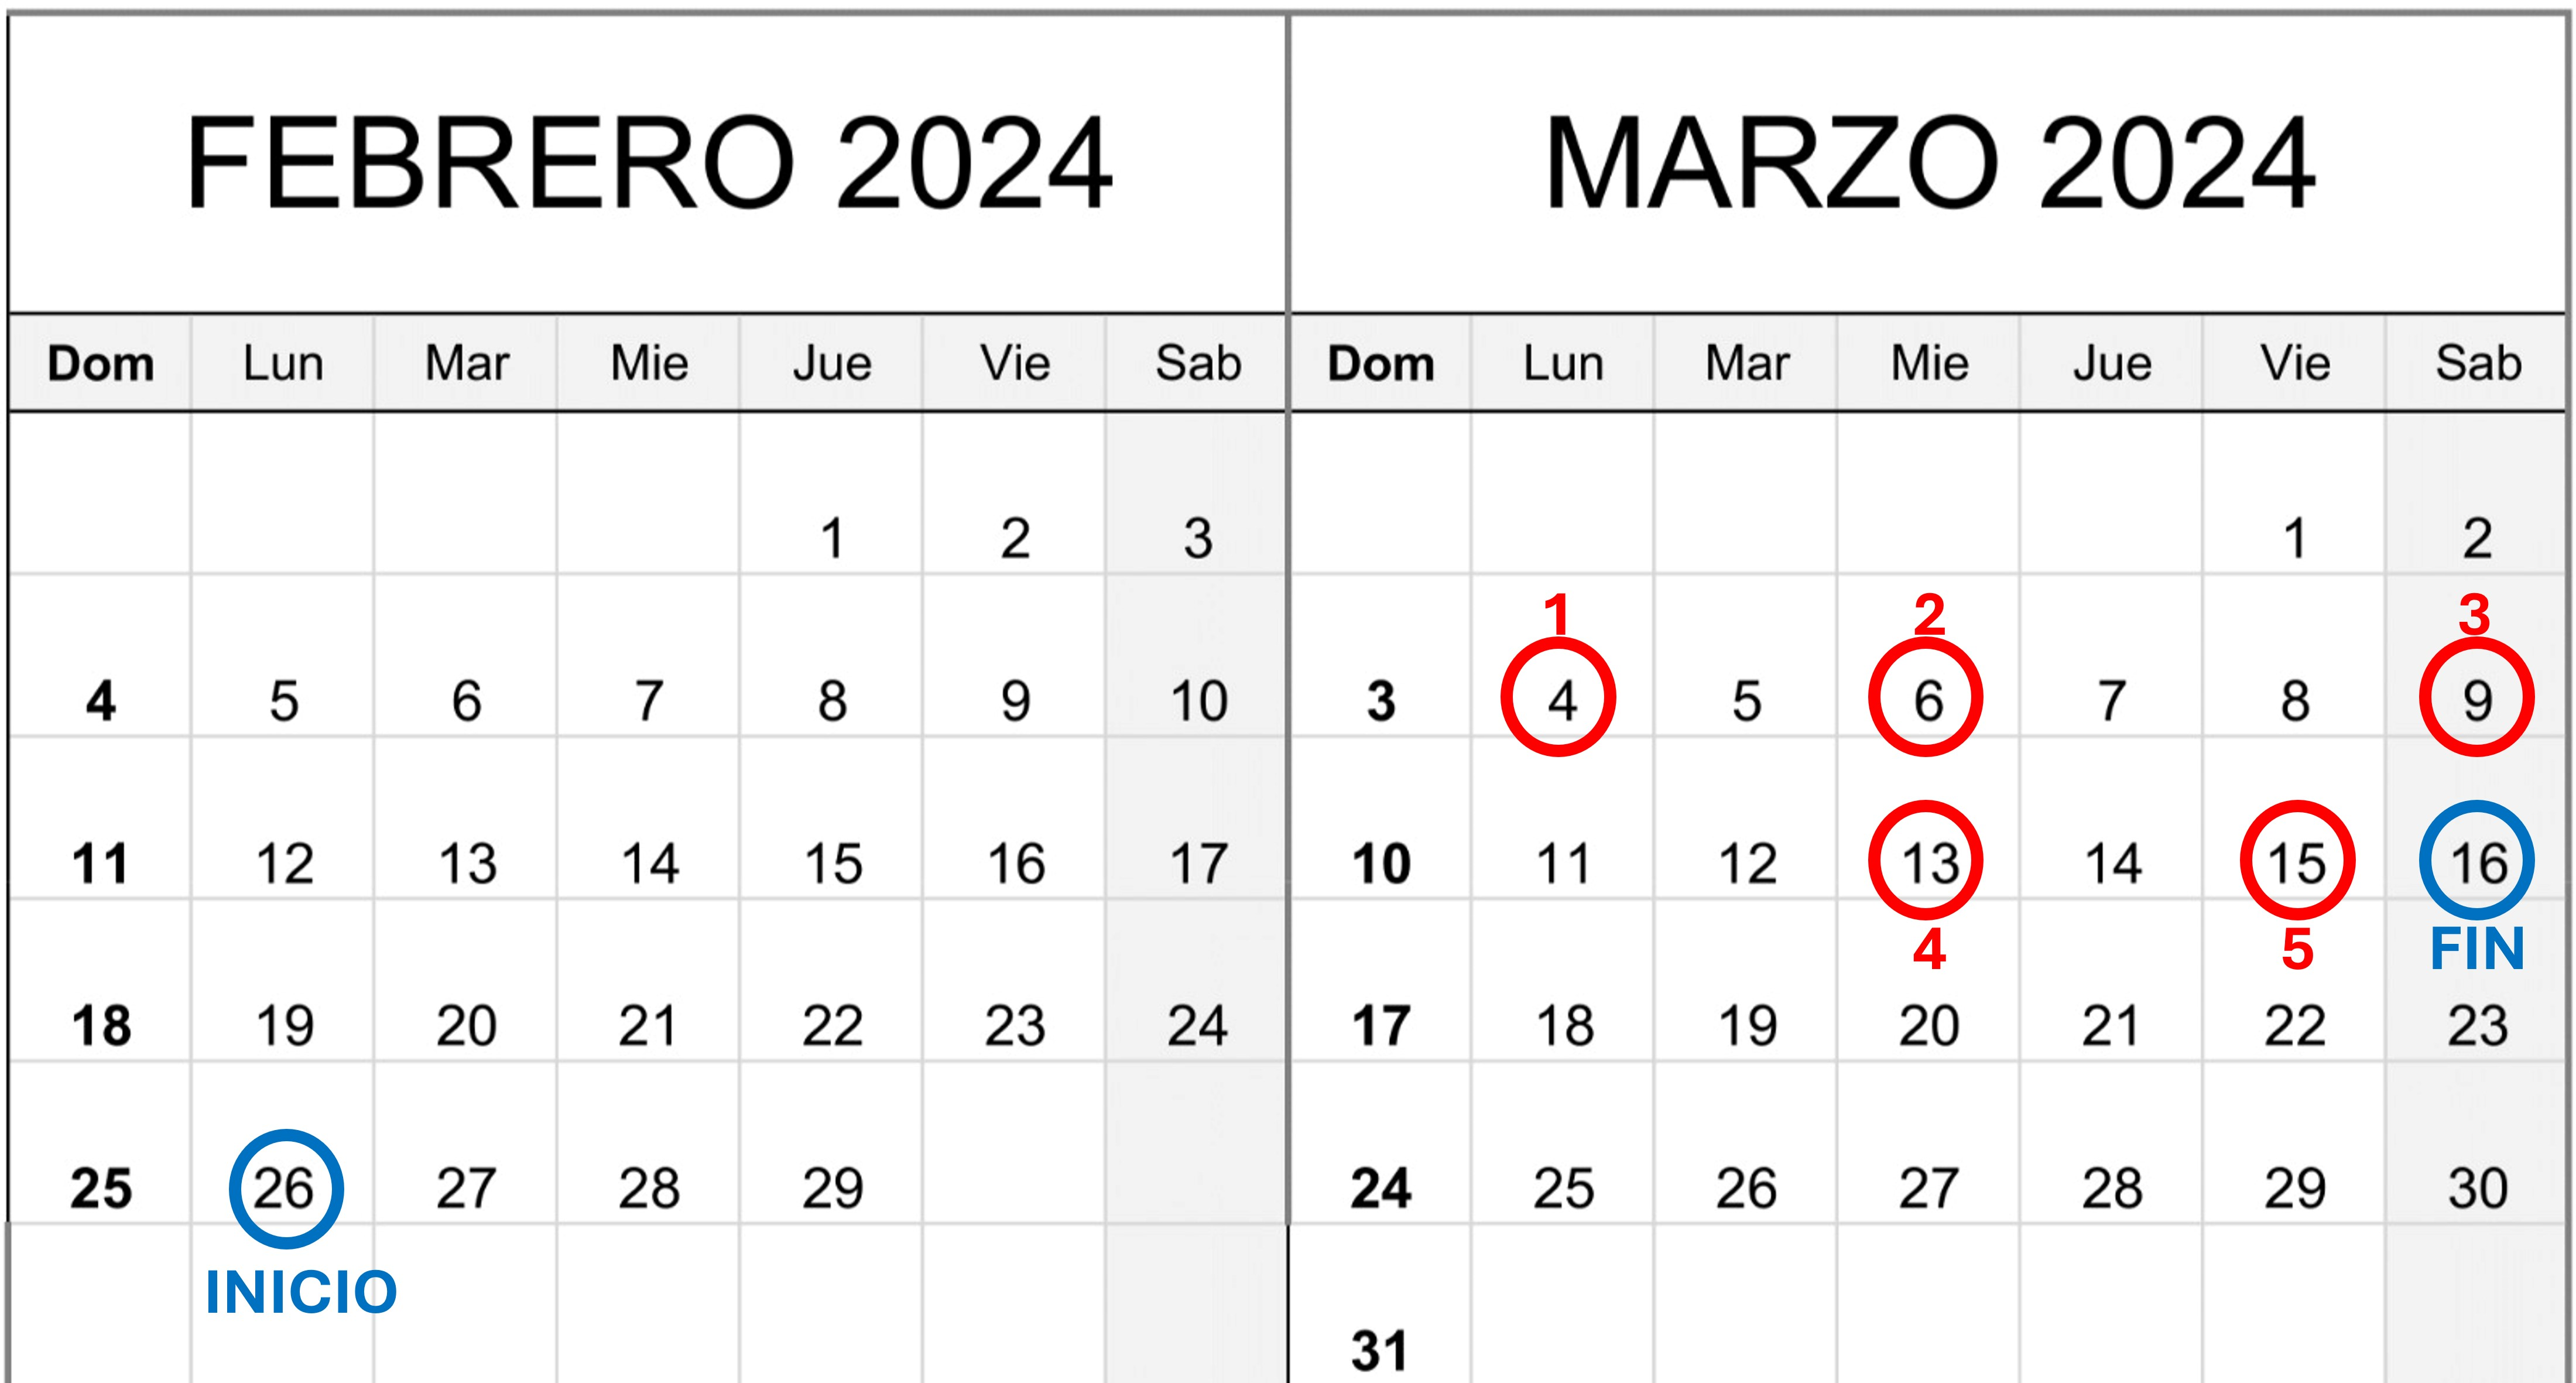
\includegraphics[width=.9\textwidth]{media/calendarizacion.jpg}
    \caption{Calendarización física de las actividades.}
    \label{fig:calendarización}
\end{figure}

\begin{enumerate}
    \item Creación del código inicial del programa. 
    \item Modificación del código del programa.
    \item Término del trabajo escrito.
    \item Código final del programa realizado.
    \item Término del manual de usuario.
    \item Término de la documentación.
\end{enumerate}

Sin embargo, el flujo de trabajo se puede desmenuzar aún más mediante el registro en el flujo de culminación de ciertas actividades más concretas.

\begin{itemize}
    \item \textbf{04/03/2024}\\Creación del archivo de código colaborativo en la plataforma \textit{Replit}.\\Creación del principal medio de comunicación entre los integrantes del equipo.\\Planeación de la lógica del programa.\\Creación del archivo colaborativo {\LaTeX} mediante la aplicación en línea \textit{OverLeaf}.
    \item \textbf{05/03/2024}\\Creación de clases \textit{Sistema}, \textit{Alumnos}, \textit{Profesores}, \textit{Materias}, \textit{Grupos} y \textit{Sistema\_de\_inscripcion}, declaración de sus atributos.\\Planeación de colecciones utilizadas.
    \item \textbf{06/03/2024}\\Desarrollo de las primeras definiciones de los programas.\\Entrega de primer avance del proyecto.
    \item \textbf{07/03/2024}\\Investigación de las colecciones en Java en sitios de internet.
    \item \textbf{08/03/2024}\\Invetigación de colecciones en Java a partir de la API.
    \item \textbf{09/03/2024}\\Finalización del trabajo escrito (investigación colecciones en Java).
    \item \textbf{10/03/2024}\\Rediseño de las colecciones en el programa. Solución programación circular.\\Creación de la clase \textit{Admin}.\\Definición de los menús individuales de cada clase.
    \item \textbf{13/03/2024}\\Definición del resto del programa, clase sistema.
    \item \textbf{15/03/2024}\\Realización del manual de usuario.
    \item \textbf{16/03/2024}\\Realización de la documentación.
\end{itemize}
    
\end{document}

